% 4.3 Siting logic: why Visakhapatnam? Added after the first draft. Extends Case 2 of O2 (sec:cases).
% Sources: public statements, official documents and press only (refs.bib: afp2026, google2026env, mongabay2026,
% scroll2026, tnm2026, newsminute2025, csm2026, niti2026, theprint2026, ceew2026, deccan2025, bs2026, googlewater2026).
% Our numbers: report/analysis/fig_siting.py -> figs/o2_siting.pdf, data/o2_siting_airwater.csv; logged in claims_report.csv (4.3).
\subsection{Siting logic: why Visakhapatnam?}\label{sec:siting}

Case~2 (Section~\ref{sec:cases}) leaves a question that the water data cannot answer. If Visakhapatnam is already
short of water, why was it chosen? We ask three things. What reasons did the project's backers give? Did water stress, the
distance to the water source or the people living nearby enter the decision? And was there a framework that required them
to? We rely on public statements, official documents and press reports only, so we can say what was stated and what is on
the record, not what was weighed in private.

\paragraph{The stated reasons are connectivity, power, talent and policy} Google told AFP that it looks for proximity to
customers and users, access to talent, potential for new clean energy and partnerships with local communities, and that
Visakhapatnam is ``one of the few places where all of these come together''; the coast also lets undersea cables reach
Australia and South Africa, making Andhra Pradesh ``India's third major subsea hub'' \citep{afp2026}. The
company's own announcement presents the cable gateway as route diversity beside the existing landings in Mumbai and Chennai
\citep{google2025}. The state added fiscal reasons: a 25\% discount on land, a 25\% discount on the price of industrial water
supply, exemption from electricity duty and a lower power tariff \citep{newsminute2025}, which the Wall Street Journal values at about
US\$2.3 billion over 20 years \citep{csm2026}. Scale matters too. India's installed data-centre capacity was about 1.5\,GW in
mid-2025 \citep{ceew2026}, so a 1\,GW hub is equal to two-thirds of it. Nor is the hub one site: it is planned on three
campuses, at Tarluvada, Adavivaram and Rambilli \citep{deccan2025}. Our case study uses Tarluvada, where the foundation stone was laid.

\paragraph{Water came in as a design input, not as a siting test} Google says independent assessments of grid stability,
power supply, water risk, ecology and noise are made 12 to 24 months before a project starts, and that the water assessment for
Visakhapatnam ``pointed to pressure on the local watershed'', which ``shaped our choice of cooling configuration from the
outset'': advanced air cooling instead of water \citep{afp2026}. That fits Google's published water-risk framework, which
rates a site's watershed for scarcity and depletion and turns to air cooling or recycled water where risk is high
\citep{google2026env}. Three things follow. First, the selection criteria Google listed to AFP do not name water; the water finding is
reported as acting on the cooling design, not on the location. Second, none of it can be checked. Google reports water use
only for fully operational sites \citep{csm2026}, and the environmental clearance discloses neither the water used in operation nor its source
\citep{mongabay2026}. Petitioners call the assessments ``inadequate'' \citep{bs2026}; we cannot confirm or refute that.
Third, the state treats water as a price: a discount, and a promise of supply by dedicated pipeline from the Polavaram
project, about 190\,km away in a straight line. An assessment of the \emph{local} watershed says nothing about water
drawn from elsewhere, whether for non-cooling needs or at the power plants (Section~\ref{sec:o2}).

\paragraph{Water stress was seen, but as a risk to manage} The record is mixed. By the Aqueduct measure Visakhapatnam is not an
extreme site: its basin is medium--high (20--40\%), with no month in which withdrawals exceed supply, and basins hosting
37.5\% of the planned capacity in our sample are less stressed while 38.6\% are more stressed (\Fig{fig:siting}a). But the
city already receives 410 of the 480 million litres a day it needs, and the district had the lowest groundwater availability in
the state (2.12\,TMC) on 1 April 2026 \citep{scroll2026}. Across India, a CEEW study found that most industry stakeholders rate water risk as low to medium, even though data
centres cluster in Mumbai, Hyderabad, Chennai and Bengaluru, where urban water demand is already high \citep{ceew2026}.
Water stress is therefore \emph{seen}, but as one risk among several rather than a reason to choose another place.

\begin{figure}[t]\centering
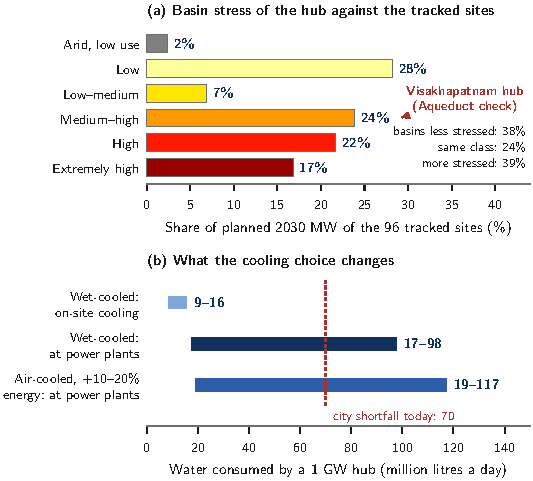
\includegraphics[width=\linewidth]{figs/o2_siting.pdf}
\caption{(a) Planned 2030 MW of the 96 tracked sites by Aqueduct baseline water-stress class, with the class of the Visakhapatnam
hub's basin (our check at Tarluvada; the hub is not in the Epoch data). (b) Water consumed by a 1\,GW hub with the Section~\ref{sec:methods}
model (low--high range): on-site cooling if wet-cooled; the water evaporated at the power plants; and the same if air cooling
needs 10--20\% more energy. Dashed line: the city's shortfall today (480 minus 410 million litres a day). US-derived grid
factors; the load factor is our assumption.}
\label{fig:siting}
\end{figure}

\paragraph{Distance and population are not criteria anywhere} We found no framework, statement or document in which the distance from a
site to its water source or the number of people nearby is a stated test. Distance enters only through the pipeline. Population
enters through public process, and there the record is thin: Mongabay India quotes a campaigner saying that data centres are being appraised as
building or township projects, which need neither a public hearing nor a draft environmental impact report. The State Environment
Impact Assessment Authority cleared the Tarluvada project on 18 April 2026, nine days after the application \citep{mongabay2026,tnm2026}. The News Minute
adds that the clearance itself records that nearly 90\% of the Tarluvada site lies in a reserve forest \citep{tnm2026}.

\begin{table*}[t]\centering
\caption{Instruments that could have governed the siting of the Visakhapatnam hub, and whether they tested water.}
\label{tab:frameworks}
\footnotesize\renewcommand{\arraystretch}{1.1}
\begin{tabular}{@{}P{3.6cm}P{4.4cm}P{8.3cm}@{}}
\toprule
Instrument & Status when the site was chosen & What it asks about water and siting \\
\midrule
Draft National Data Centre Policy (MeitY, 2020) & Never notified & No binding environmental requirement
\citep{mongabay2026} \\
State data-centre policies (15 states) & In force & Most set no PUE or WUE standard \citep{mongabay2026} \\
Environmental clearance (EIA Notification 2006) & Applied (18 April 2026) & Appraised as a building or township project (as reported): no public hearing;
operating water use and source not disclosed \citep{mongabay2026,tnm2026} \\
Google's water-risk framework & Company-internal; results not published & Rates the local watershed; high risk points to
air cooling or recycled water \citep{google2026env,afp2026} \\
NITI Aayog and Deloitte \emph{Data Centre Evaluation Framework} & Released 14 October 2026, after approval and groundbreaking; advisory
& Five pillars, including water and siting. A 20--30-year seasonal water balance for each catchment, including farming; ``red zones''
for water stress; MeitY audit; states apply it \citep{niti2026,theprint2026} \\
\bottomrule
\end{tabular}
\end{table*}

\paragraph{Frameworks exist, but none was in force in time} Several exist (\Tab{tab:frameworks}), but none was binding when the site was chosen, and the only
one that tests catchment water, the NITI Aayog evaluation framework, arrived in October 2026, six months after the clearance
and the groundbreaking. Visakhapatnam was not judged against it. Its tests are the ones this section found missing: a water
balance that counts competing users, restricted zones where stress is high, and checks on who benefits.

\paragraph{What the cooling choice changes} Air cooling does remove the water that would be evaporated on site. By our
model that is 9--16 million litres a day for 1\,GW, 2--4\% of the city's present supply (\Fig{fig:siting}b). But air cooling needs more
electricity, about 10\% on average and roughly twice that on a hot day by Google's own figure \citep{googlewater2026}, and
most of the hub's water is used at the power plants anyway. With 10--20\% more energy the water at the power plants rises by 2--20
million litres a day, so the net effect on all water consumed lies between a saving of 7 and an increase of 4 million litres a day. In
Google's words, ``it becomes a tradeoff between reducing stress on the grid versus reducing stress on the watershed''
\citep{googlewater2026}. Air cooling therefore mostly \emph{moves} the water from the city to the power stations, and the
carbon to the grid. It protects the town's taps, which matters locally, but it is not a net water saving.

\begin{reading}
Our reading: on the public record, connectivity, power, land and incentives chose the site, and water was handled afterwards,
through the choice of cooling, a pledge to replenish, and a pipeline. That is a defensible design response, and the site is not
the most stressed in our sample. But it leaves the questions a water-first screen would ask (distance to source, competing
users, the people nearby) unanswered in public, and no framework in force required them. A comparison with Mumbai, Chennai,
Hyderabad and Bengaluru would show whether Visakhapatnam was the better water choice among Indian options.
\end{reading}

\begin{finding}{Finding 4. Water shaped how Visakhapatnam will be cooled, not whether it was chosen}
On the public record the site was chosen for cables, power, land and incentives; water risk acted on the cooling design.
Distance to source and nearby population are tests in no instrument in force at the time, and the first framework that
asks for a catchment water balance (NITI Aayog, October 2026) came after the clearance. Air cooling shifts, rather than removes,
the hub's water: net change between $-7$ and $+4$ million litres a day.
\end{finding}
